% Exam Template for UMTYMP and Math Department courses
%
% Using Philip Hirschhorn's exam.cls: http://www-math.mit.edu/~psh/#ExamCls
%
% run pdflatex on a finished exam at least three times to do the grading table on front page.
%
%%%%%%%%%%%%%%%%%%%%%%%%%%%%%%%%%%%%%%%%%%%%%%%%%%%%%%%%%%%%%%%%%%%%%%%%%%%%%%%%%%%%%%%%%%%%%%

% These lines can probably stay unchanged, although you can remove the last
% two packages if you're not making pictures with tikz.
\documentclass[11pt]{exam}
\RequirePackage{amssymb, amsfonts, amsmath, latexsym, verbatim, xspace, setspace}
\usepackage{graphicx}
\usepackage{multicol}

% By default LaTeX uses large margins.  This doesn't work well on exams; problems
% end up in the "middle" of the page, reducing the amount of space for students
% to work on them.
\usepackage[margin=1in]{geometry}


% Here's where you edit the Class, Exam, Date, etc.
\newcommand{\class}{It's About Time}
\newcommand{\term}{Colorado State Finals 2015}
\newcommand{\examdate}{April 18, 2015}
\newcommand{\timelimit}{30 Minutes}
\newcommand{\unit}[1]{\ensuremath{\, \mathrm{#1}}}

% For an exam, single spacing is most appropriate
\singlespacing
% \onehalfspacing
% \doublespacing

% For an exam, we generally want to turn off paragraph indentation
\parindent 0ex

\begin{document} 

% These commands set up the running header on the top of the exam pages
\pagestyle{head}
\firstpageheader{}{}{}
\runningheader{\class}{Page \thepage\ of \numpages}{\examdate}
\runningheadrule

\begin{flushright}
\begin{tabular}{p{2.8in} r l}
\textbf{\class} & \textbf{School Name} & \makebox[2in]{\hrulefill}\\
\textbf{\term} & \textbf{Team Number} & \makebox[2in]{\hrulefill}\\
\textbf{\examdate} & \textbf{Name (Print):} & \makebox[2in]{\hrulefill}\\
\textbf{Time Limit: \timelimit} & \textbf{Name (Print):} & \makebox[2in]{\hrulefill}\\
\end{tabular}\\
\end{flushright}
\rule[1ex]{\textwidth}{.1pt}


This exam contains \numpages\ pages (including this cover page) and
\numquestions\ problems.  Check to see if any pages are missing.  Enter
all requested information on the top of this page, and put your initials
on the top of every page, in case the pages become separated.\\

You may only use your books, notes, or any calculator on this exam.\\

You are required to show your work on each problem on this exam.  

\begin{minipage}[t]{3.7in}
\vspace{0pt}
\begin{itemize}

\item \textbf{Organize your work}, in a reasonably neat and coherent way, in
the space provided. Work scattered all over the page without a clear ordering will 
receive very little credit.  

\item \textbf{Mysterious or unsupported answers will not receive full
credit}.  A correct answer, unsupported by calculations, explanation,
or algebraic work will receive no credit; an incorrect answer supported
by substantially correct calculations and explanations might still receive
partial credit.

\item If you need more space, use the back of the pages; clearly indicate when you have done this.
\end{itemize}

Do not write in the table to the right.
\end{minipage}
\hfill
\begin{minipage}[t]{2.3in}
\vspace{0pt}
%\cellwidth{3em}
\gradetablestretch{2}
\vqword{Problem}
\addpoints % required here by exam.cls, even though questions haven't started yet.	
\gradetable[v]%[pages]  % Use [pages] to have grading table by page instead of question

\end{minipage}
\newpage % End of cover page

%%%%%%%%%%%%%%%%%%%%%%%%%%%%%%%%%%%%%%%%%%%%%%%%%%%%%%%%%%%%%%%%%%%%%%%%%%%%%%%%%%%%%
%
% See http://www-math.mit.edu/~psh/#ExamCls for full documentation, but the questions
% below give an idea of how to write questions [with parts] and have the points
% tracked automatically on the cover page.
%
%
%%%%%%%%%%%%%%%%%%%%%%%%%%%%%%%%%%%%%%%%%%%%%%%%%%%%%%%%%%%%%%%%%%%%%%%%%%%%%%%%%%%%%

\begin{questions}
\addpoints

% Basic question
\question[8]\textbf{Matching:} Fill in the correct clock type into the table below
\addpoints

\begin{center}
\Large
Clock Types\\
\normalsize
$\bullet$ Cesium Fountain \ \ \ \ $\bullet$ Cesium Beam \ \ \ \ $\bullet$ Harrison Chronometer \ \ \ \ \ \ $\bullet$ Optical Lattice\\
$\bullet$ Pendulum Clock \ \ \ \ \ $\bullet$ Quartz Crystal \ \ \ \ \ \ $\bullet$ Sundial \ \ \ \ $\bullet$ Water Clock
\end{center}

\begin{center}
\Large
\begin{tabular}{|c|c|c|}
\hline
Year of         &Timing Uncertainty         &          \\        
Invention       &Uncertainty (24h)          &Clock Type\\
\hline 
$\approx$3500 BC        &N/A                               &\hspace*{3.5in}\\
\hline 
$\approx$1600 BC        &$>30\unit{min}$                   &\hspace*{3.5in}\\
\hline
1656 AD                 &$10\unit{s}$                      &\hspace*{3.5in}\\
\hline
1759 AD                 &$350\unit{ms}$                    &\hspace*{3.5in}\\
\hline
1927 AD                 &$10\unit{\mu s}$                 &\hspace*{3.5in}\\
\hline
1952 AD                 &$1\unit{ns}$                      &\hspace*{3.5in}\\
\hline
1991 AD                 &$100\unit{ps}$                    &\hspace*{3.5in}\\
\hline
2014 AD                 &$10\unit{ps}$                     &\hspace*{3.5in}\\
\hline
\end{tabular} 
\end{center}

\normalsize

\addpoints
\question[2]\textbf{Short Answer:} The quantity that measures the ratio between the rate an oscillator losses energy to the amount of energy it stores is called...
\vspace{1in}

\addpoints
\question[5]\textbf{Short Answer:} Two events are separated by a positive \emph{spacetime interval}, $\Delta s$, (note we are using the space-like convention) it is said that is interval is...
\vspace{1in}

\addpoints
\question[5]\textbf{Short Answer:} A pendulum's period is constant and given by the equation
$$T=2\pi\sqrt{\frac{L}{g}}$$
if the angle of deflection $\theta$ is...
\vspace{1in}

\newpage
\addpoints
\question[5]\textbf{Matching:} Match the time signal in blue, $f(t)$, with the spectrum or \emph{Fourier transform}, $F(\omega)$.
\Large
\begin{center}
\begin{tabular}{|c|c|}
\hline
$f(t)$     &$F(\omega)$\\
\hline
(1)          &\hspace*{1in}\\
\hline
(2)          &\hspace*{1in}\\
\hline
(3)          &\hspace*{1in}\\
\hline
(4)          &\hspace*{1in}\\
\hline
(5)          &\hspace*{1in}\\
\hline
\end{tabular}
\end{center}

\normalsize
\begin{multicols}{2} 
(1)\\
(2)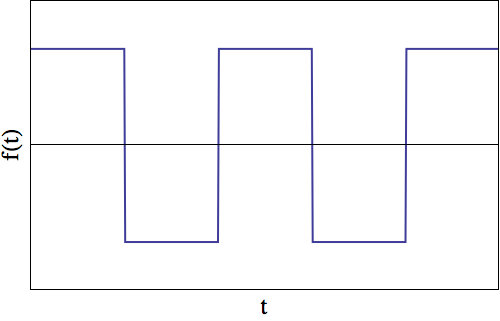
\includegraphics[width=0.3\textwidth]{Square.png}\\
(3)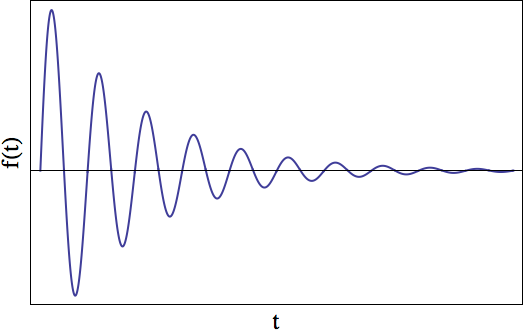
\includegraphics[width=0.3\textwidth]{Damped.png}\\
(4)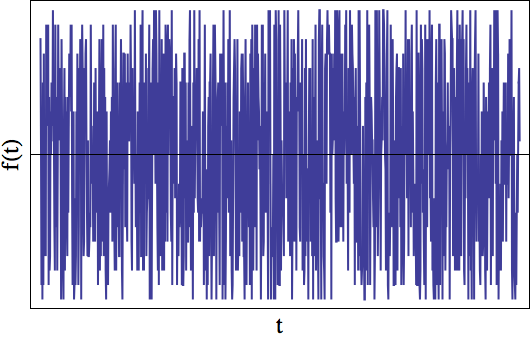
\includegraphics[width=0.3\textwidth]{Noise.png}\\
(5)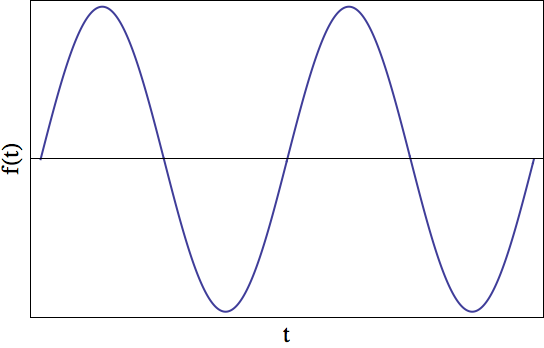
\includegraphics[width=0.3\textwidth]{SINE.png}\\
\hspace*{0.18in}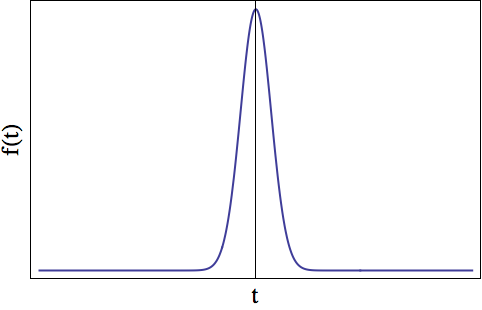
\includegraphics[width=0.3\textwidth]{Gauss.png}\\

\columnbreak

(a)\\
(b)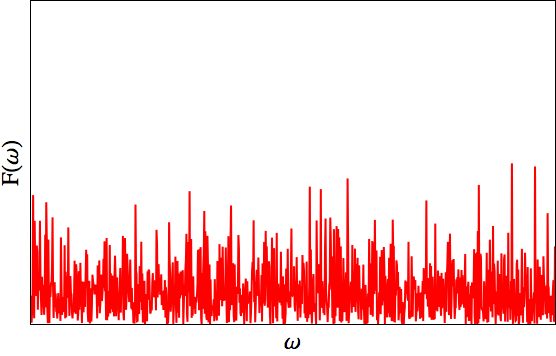
\includegraphics[width=0.3\textwidth]{FT_Noise.png}\\
(c)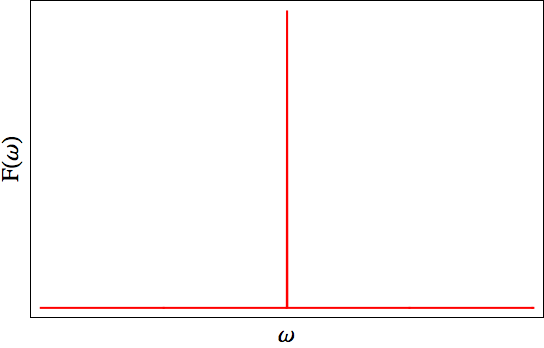
\includegraphics[width=0.3\textwidth]{FT_SINE.png}\\
(d)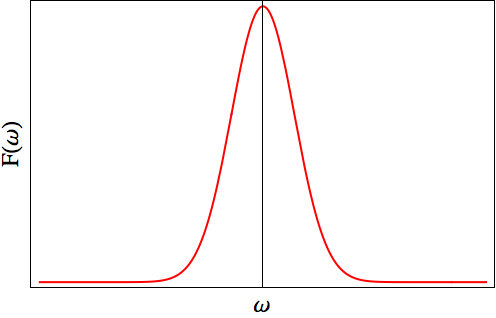
\includegraphics[width=0.3\textwidth]{FT_Gauss.png}\\
(e)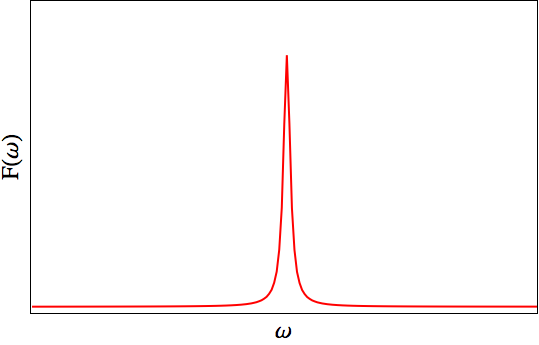
\includegraphics[width=0.3\textwidth]{FT_Damped.png}\\
\hspace*{0.18in}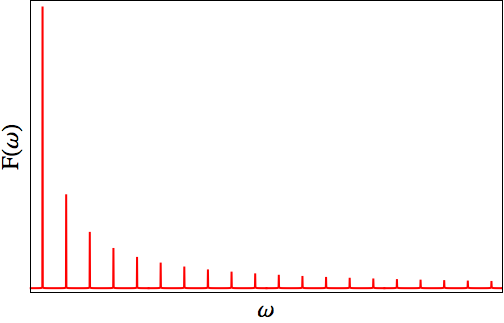
\includegraphics[width=0.3\textwidth]{FT_Square.png}\\
\end{multicols}

\newpage
\addpoints
\question[5]\textbf{Calculation:}
\noaddpoints
\begin{parts}
\part[3] A time synchronization signal is sent between two clocks separated by a distance of $5500\unit{km}$. Assuming the signal travels at the speed of light what is the amount of time you need to adjust to account for the delay?
\vspace{4.5in}
\part[2] What is the delay if the signal travels in an optical fiber with and index of refraction $n=1.5$?
\vspace{4.5in}
\end{parts}

\newpage
\addpoints
\question[5]\textbf{Calculation:} You are timing the period of a pendulum with a stopwatch. The primary source of uncertainty is human reaction time with an error of $\sigma=\pm0.1\unit{s}$. Which measurement has lower uncertainty taking ten averages of a single period or measuring ten periods at once and dividing by ten? 
\vspace{4.5in}

\addpoints
\question[5]\textbf{Calculation:} You travel from earth to the center of the galaxy and back at the speed of light (without accelerating). An observer on earth waits $50\unit{yrs}$ for you to return. How long does the trip appear to you?
\vspace{4.5in}

\newpage
\addpoints
\question[5]\textbf{Calculation:} Matthew McConaughey is on a planet that is orbiting a black hole. Mr. McConaughey spends $1\unit{hr}$ on the surface of the planet and once he returns to his space station that is a long distance from the black hole he has found that $1\unit{yr}$ has passed. Assume the planet orbits at a radius of $r=1.5\times10^8\unit{km}$ and that the travel was instant. What was the mass of the black hole? 
\vspace{4.5in}

\newpage
\addpoints
\question[5]\textbf{Calculation(Tiebreaker):} A massless spring with one end fixed and with a mass, $m$ attached to the free end (see figure). Assume the spring obeys \emph{Hooke's Law} ($F=-kx$) and the surface the mass is resting on is frictionless. 
\noaddpoints

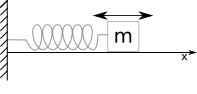
\includegraphics[width=0.5\textwidth]{Spring.png}

\begin{parts}
\part[3]
Show that $x(t) = A\sin(\omega_0t)$ is a solution for the equations of motion for the mass.  Note that $\omega_0 = \sqrt{k/m}$.
\vspace{4.5in}

\part[2]
What are the units of $\omega_0$?
\vspace{4.5in}
\end{parts}
\end{questions}
\end{document}
